% answers.tex —— 2007 年·普通高等学校招生考试·江西卷·理科 · 参考答案与详细解析片段
% 由 tools/generate_projects.py 依来源总账自 2007/2007_数学真题_江西理_试题.md + 2007/2007_数学真题_江西理_解析正文.md + 2007/2007_数学真题_江西理_答案要点.md 生成，勿手改（改源 MD 后重跑）


\begin{gktip}
固定候选 PDF 仅含题面，无答案、解析和评分标准，原卷亦未标注分值；以下为非官方编者独立推导，官方答案字段为空。来源发布者、出版者、版次与官方身份均未核。
\end{gktip}

\begin{answer}
\gksolhead{1}{}

\textbf{题目}：

化简 $\dfrac{2+4\mathrm i}{(1+\mathrm i)^2}$ 的结果是（　）

（A）$2+\mathrm i$

（B）$-2+\mathrm i$

（C）$2-\mathrm i$

（D）$-2-\mathrm i$

\Needspace{4\baselineskip}
\textbf{解析}

\nopagebreak[4]
\[(1+\mathrm i)^2=2\mathrm i,\]

\nopagebreak[4]
\[\frac{2+4\mathrm i}{2\mathrm i}=\frac{2+4\mathrm i}{2\mathrm i}\cdot\frac{-\mathrm i}{-\mathrm i}=\frac{(2+4\mathrm i)(-\mathrm i)}{2}=\frac{4-2\mathrm i}{2}=2-\mathrm i.\]

\gkanswer{答案：C。}

\end{answer}
\begin{answer}
\gksolhead{2}{}

\textbf{题目}：

$\lim\limits_{x\to1}\dfrac{x^3-x^2}{x-1}$（　）

（A）等于 $0$

（B）等于 $1$

（C）等于 $3$

（D）不存在

\Needspace{4\baselineskip}
\textbf{解析}

\nopagebreak[4]
\[\frac{x^3-x^2}{x-1}=x^2\quad(x\neq1),\]

故极限为 $1$。

\gkanswer{答案：B。}

\end{answer}
\begin{answer}
\gksolhead{3}{}

\textbf{题目}：

若 $\tan\left(\dfrac{\pi}{4}-\alpha\right)=3$，则 $\cot\alpha$ 等于（　）

（A）$-2$

（B）$-\frac12$

（C）$\frac12$

（D）$2$

\Needspace{4\baselineskip}
\textbf{解析}

\nopagebreak[4]
\[\tan\left(\frac{\pi}{4}-\alpha\right)=\frac{1-\tan\alpha}{1+\tan\alpha}=3.\]

\Needspace{5\baselineskip}
解得

\nopagebreak[4]
\[1-\tan\alpha=3+3\tan\alpha\ \Rightarrow\ \tan\alpha=-\frac12,\]

\Needspace{5\baselineskip}
故

\nopagebreak[4]
\[\cot\alpha=-2.\]

\gkanswer{答案：A。}

\end{answer}
\begin{answer}
\gksolhead{4}{}

\textbf{题目}：

已知 $\left(\sqrt x+\dfrac{3}{\sqrt[3]{x}}\right)^n$ 展开式中，各项系数的和与其各项二项式系数的和之比为 $64$，则 $n$ 等于（　）

（A）$4$

（B）$5$

（C）$6$

（D）$7$

\Needspace{4\baselineskip}
\textbf{解析}

\Needspace{5\baselineskip}
各项系数和令 $x=1$：

\nopagebreak[4]
\[(1+3)^n=4^n.\]

\Needspace{5\baselineskip}
二项式系数和为 $2^n$。由题意

\nopagebreak[4]
\[\frac{4^n}{2^n}=2^n=64,\]

故 $n=6$。

\gkanswer{答案：C。}

\end{answer}
\begin{answer}
\gksolhead{5}{}

\textbf{题目}：

若 $0<x<\dfrac{\pi}{2}$，则下列命题中正确的是（　）

（A）$\sin x<\frac3\pi x$

（B）$\sin x>\frac3\pi x$

（C）$\sin x<\frac4{\pi^2}x^2$

（D）$\sin x>\frac4{\pi^2}x^2$

\Needspace{4\baselineskip}
\textbf{解析}

\Needspace{5\baselineskip}
设 $h(x)=\sin x-\dfrac4{\pi^2}x^2$。在 $\left(0,\dfrac{\pi}{2}\right)$ 上可验证 $h(x)>0$（端点 $h(0)=h\left(\dfrac{\pi}{2}\right)=0$，中间为正），故

\nopagebreak[4]
\[\sin x>\frac4{\pi^2}x^2.\]

其余选项在 $x=\dfrac{\pi}{2}$ 或 $x\to0^+$ 处不成立。

\gkanswer{答案：D。}

\end{answer}
\begin{answer}
\gksolhead{6}{}

\textbf{题目}：

若集合 $M=\{0,1,2\}$，$N=\{(x,y)\mid x-2y+1\geqslant0$ 且 $x-2y-1\leqslant0$，$x$，$y\in M\}$，则 $N$ 中元素的个数为（　）

（A）$9$

（B）$6$

（C）$4$

（D）$2$

\Needspace{4\baselineskip}
\textbf{解析}

\Needspace{5\baselineskip}
条件等价于

\nopagebreak[4]
\[-1\leqslant x-2y\leqslant1.\]

逐点检验 $(x,y)\in\{0,1,2\}^2$：

\begin{itemize}
\item $y=0$：$x=0,1$；
\item $y=1$：$x=1,2$；
\item $y=2$：无。
\end{itemize}

共 $4$ 个，选 C。

\gkanswer{答案：C。}

\end{answer}
\begin{answer}
\gksolhead{7}{}

\textbf{题目}：

如图，正方体 $AC_1$ 的棱长为 $1$，过点 $A$ 作平面 $A_1BD$ 的垂线，垂足为点 $H$。则以下命题中，错误的是（　）
\nopagebreak[4]
\begin{center}% 2007 年江西卷理科第 7 题：棱长为 1 的正方体 AC1，AH⊥平面 A1BD，H 为垂足。
%   图中标出 A、B、C、D、A1、B1、C1、D1、H 与平面 A1BD。
% 来源 PDF：gaokaomath-src/普通高考/2007/2007江西理.pdf
% SHA-256：6602cbc393b02e9940beb0035be6e2a28d88a77e0e7792260dcd4c873b542a82
% 原页：2007江西理.pdf 第 1 页（A3 三栏）第 3 栏，书页码 385。
% 重绘依据：按原页正方体斜投影、平面 A1BD 与垂足 H 的位置重绘。
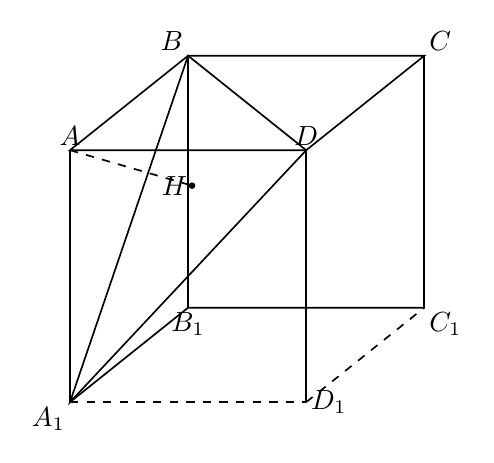
\begin{tikzpicture}[scale=1.0, semithick,
  every node/.style={inner sep=1.5pt}]

  \coordinate (A)  at (0,3.2);
  \coordinate (B)  at (1.5,4.4);
  \coordinate (C)  at (4.5,4.4);
  \coordinate (D)  at (3.0,3.2);
  \coordinate (A1) at (0,0);
  \coordinate (B1) at (1.5,1.2);
  \coordinate (C1) at (4.5,1.2);
  \coordinate (D1) at (3.0,0);

  % 被遮挡的棱
  \draw[dashed] (A1) -- (D1);
  \draw[dashed] (D1) -- (C1);
  \draw[dashed] (D1) -- (D);

  % 可见的棱
  \draw (A) -- (B) -- (C) -- (D) -- cycle;
  \draw (A) -- (A1);
  \draw (B) -- (B1);
  \draw (C) -- (C1);
  \draw (D) -- (D1);
  \draw (A1) -- (B1) -- (C1);

  % 平面 A1BD 与垂足 H
  \draw (A1) -- (B) -- (D) -- cycle;
  \coordinate (H) at (1.55,2.75);
  \draw[dashed] (A) -- (H);
  \fill (H) circle (1.2pt);

  \node[above] at (A) {$A$};
  \node[above left] at (B) {$B$};
  \node[above right] at (C) {$C$};
  \node[above] at (D) {$D$};
  \node[below left] at (A1) {$A_1$};
  \node[below] at (B1) {$B_1$};
  \node[below right] at (C1) {$C_1$};
  \node[right] at (D1) {$D_1$};
  \node[left] at (H) {$H$};
\end{tikzpicture}
\end{center}
\nopagebreak[4]
（A）点 $H$ 是 $\triangle A_1BD$ 的垂心

（B）$AH$ 垂直平面 $CB_1D_1$

（C）$AH$ 的延长线经过点 $C_1$

（D）直线 $AH$ 和 $BB_1$ 所成的角为 $45^\circ$

\Needspace{4\baselineskip}
\textbf{解析}

\Needspace{5\baselineskip}
以 $A$ 为原点建系（同第 16 题），$AH$ 的方向向量为 $(1,1,1)$，$BB_1$ 的方向向量为 $(0,0,1)$。设夹角为 $\varphi$，则

\nopagebreak[4]
\[\cos\varphi=\frac1{\sqrt3},\]

\nopagebreak[4]
\[\varphi=\arccos\frac1{\sqrt3}\approx54.7^\circ\neq45^\circ.\]

前三项均正确，故选 D。

\gkanswer{答案：D。}

\end{answer}
\begin{answer}
\gksolhead{8}{}

\textbf{题目}：

四位好朋友在一次聚会上，他们按照各自的爱好选择了形状不同、内空高度相等、杯口半径相等的圆口酒杯，如图所示，盛满酒后他们约定：先各自饮杯中酒的一半。设剩余酒的高度从左到右依次为 $h_1$，$h_2$，$h_3$，$h_4$，则它们的大小关系正确的是（　）
\nopagebreak[4]
\begin{center}% 2007 年江西卷理科第 8 题：四个形状不同、内空高度与杯口半径相等的圆口酒杯。
%   从左到右：半球形杯、圆锥形杯、圆台形杯、圆柱形杯；虚线表示剩余半杯酒的高度。
% 来源 PDF：gaokaomath-src/普通高考/2007/2007江西理.pdf
% SHA-256：6602cbc393b02e9940beb0035be6e2a28d88a77e0e7792260dcd4c873b542a82
% 原页：2007江西理.pdf 第 1 页（A3 三栏）第 2 栏，书页码 385。
% 重绘依据：按原页四种杯形与半杯液面位置重绘，高度差不按严格比例。
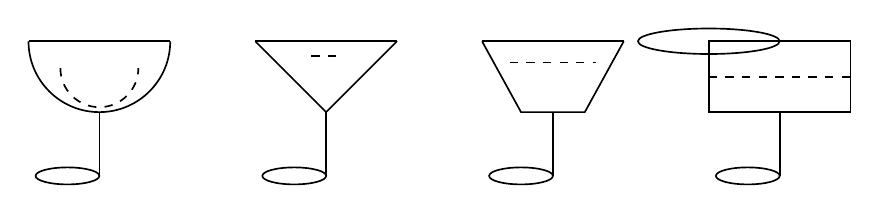
\begin{tikzpicture}[scale=0.9, semithick,
  every node/.style={inner sep=1pt}]

  % ---------------- 半球形杯 ----------------
  \begin{scope}[shift={(0,0)}]
    \draw (-1,3) arc[start angle=180,end angle=360,radius=1];
    \draw (-1,3) -- (-1,3);
    \draw (-1,3) -- (1,3);
    \draw[dashed] (-0.55,2.62) arc[start angle=180,end angle=360,radius=0.55];
    \draw (0,2) -- (0,1.1);
    \draw (-0.45,1.1) ellipse (0.45 and 0.12);
  \end{scope}

  % ---------------- 圆锥形杯 ----------------
  \begin{scope}[shift={(3.2,0)}]
    \draw (-1,3) -- (0,2) -- (1,3);
    \draw (-1,3) -- (1,3);
    \draw[dashed] (-0.21,2.79) -- (0.21,2.79);
    \draw (0,2) -- (0,1.1);
    \draw (-0.45,1.1) ellipse (0.45 and 0.12);
  \end{scope}

  % ---------------- 圆台形杯 ----------------
  \begin{scope}[shift={(6.4,0)}]
    \draw (-1,3) -- (-0.45,2) -- (0.45,2) -- (1,3);
    \draw (-1,3) -- (1,3);
    \draw[dashed] (-0.61,2.7) -- (0.61,2.7);
    \draw (0,2) -- (0,1.1);
    \draw (-0.45,1.1) ellipse (0.45 and 0.12);
  \end{scope}

  % ---------------- 圆柱形杯 ----------------
  \begin{scope}[shift={(9.6,0)}]
    \draw (-1,3) -- (1,3) -- (1,2) -- (-1,2) -- cycle;
    \draw (-1,3) ellipse (1 and 0.18);
    \draw[dashed] (-1,2.5) -- (1,2.5);
    \draw (0,2) -- (0,1.1);
    \draw (-0.45,1.1) ellipse (0.45 and 0.12);
  \end{scope}
\end{tikzpicture}
\end{center}
\nopagebreak[4]
（A）$h_2>h_1>h_4$

（B）$h_1>h_2>h_3$

（C）$h_3>h_2>h_4$

（D）$h_2>h_4>h_1$

\Needspace{4\baselineskip}
\textbf{解析}

锥形杯半杯所需高度最大，半球形杯次之，圆柱形杯为 $\dfrac H2$ 最小，故 $h_2>h_1>h_4$。

\gkanswer{答案：A。}

\end{answer}
\begin{answer}
\gksolhead{9}{}

\textbf{题目}：

设椭圆 $\dfrac{x^2}{a^2}+\dfrac{y^2}{b^2}=1$（$a>b>0$）的离心率为 $e=\dfrac12$，右焦点为 $F(c,0)$，方程 $ax^2+bx-c=0$ 的两个实根分别为 $x_1$ 和 $x_2$，则点 $P(x_1,x_2)$（　）

（A）必在圆 $x^2+y^2=2$ 内

（B）必在圆 $x^2+y^2=2$ 上

（C）必在圆 $x^2+y^2=2$ 外

（D）以上三种情形都有可能

\Needspace{4\baselineskip}
\textbf{解析}

\Needspace{5\baselineskip}
由 $e=\dfrac12$ 得 $a=2c$，$b=\sqrt3c$，方程化为

\nopagebreak[4]
\[2x^2+\sqrt3x-1=0.\]

\Needspace{5\baselineskip}
由韦达定理 $x_1+x_2=-\dfrac{\sqrt3}{2}$，$x_1x_2=-\dfrac12$，故

\nopagebreak[4]
\[x_1^2+x_2^2=\frac34+1=\frac74<2.\]

点 $P$ 在圆内。

\gkanswer{答案：A。}

\end{answer}
\begin{answer}
\gksolhead{10}{}

\textbf{题目}：

将一个骰子连续抛掷三次，它落地时向上的点数依次成等差数列的概率为（　）

（A）$\frac19$

（B）$\frac1{12}$

（C）$\frac1{15}$

（D）$\frac1{18}$

\Needspace{4\baselineskip}
\textbf{解析}

总结果 $6^3=216$。按中间点数 $b$ 计数：

\begin{itemize}
\item $b=1$：$1$ 个；
\item $b=2$：$3$ 个；
\item $b=3$：$5$ 个；
\item $b=4$：$5$ 个；
\item $b=5$：$3$ 个；
\item $b=6$：$1$ 个。
\end{itemize}

\Needspace{5\baselineskip}
共 $18$ 个，概率

\nopagebreak[4]
\[\frac{18}{216}=\frac1{12}.\]

\gkanswer{答案：B。}

\end{answer}
\begin{answer}
\gksolhead{11}{}

\textbf{题目}：

设函数 $f(x)$ 是 $\mathbf R$ 上以 $5$ 为周期的可导偶函数，则曲线 $y=f(x)$ 在 $x=5$ 处的切线的斜率为（　）

（A）$-\frac15$

（B）$0$

（C）$\frac15$

（D）$5$

\Needspace{4\baselineskip}
\textbf{解析}

\Needspace{5\baselineskip}
$f$ 以 $5$ 为周期，故 $f'(5)=f'(0)$。又 $f$ 为偶函数，$f(-x)=f(x)$，求导得 $f'(-x)=-f'(x)$，令 $x=0$ 得

\nopagebreak[4]
\[f'(0)=0.\]

故切线斜率为 $0$。

\gkanswer{答案：B。}

\end{answer}
\begin{answer}
\gksolhead{12}{}

\textbf{题目}：

设 $p$：$f(x)=\mathrm e^x+\ln x+2x^2+mx+1$ 在 $(0,+\infty)$ 内单调递增，$q$：$m\geqslant-5$，则 $p$ 是 $q$ 的（　）

（A）充分不必要条件

（B）必要不充分条件

（C）充分必要条件

（D）既不充分也不必要条件

\Needspace{4\baselineskip}
\textbf{解析}

\nopagebreak[4]
\[f'(x)=\mathrm e^x+\frac1x+4x+m.\]

记 $g(x)=\mathrm e^x+\dfrac1x+4x$，则 $p$ 等价于 $m\geqslant-\min g(x)$。可验证 $g(x)$ 在 $(0,+\infty)$ 上的最小值大于 $5$，故 $-\min g>-5$。

因此 $m\geqslant-5\Rightarrow m\geqslant-\min g$，即 $q\Rightarrow p$；反之不成立。$p$ 是 $q$ 的必要不充分条件。

\gkanswer{答案：B。}

\end{answer}
\begin{answer}
\gksolhead{13}{}

\textbf{题目}：

设函数 $y=4+\log_2(x-1)$（$x\geqslant3$），则其反函数的定义域为\gkblank{}。

\Needspace{4\baselineskip}
\textbf{解析}

\Needspace{5\baselineskip}
$x\geqslant3$ 时 $x-1\geqslant2$，故

\nopagebreak[4]
\[y=4+\log_2(x-1)\geqslant4+1=5.\]

反函数的定义域等于原函数的值域，即 $[5,+\infty)$。

\gkanswer{答案：$[5,+\infty)$。}

\end{answer}
\begin{answer}
\gksolhead{14}{}

\textbf{题目}：

已知数列 $\{a_n\}$ 对于任意 $p$，$q\in\mathbf N^*$，有 $a_p+a_q=a_{p+q}$，若 $a_1=\dfrac19$，则 $a_{36}=$\gkblank{}。

\Needspace{4\baselineskip}
\textbf{解析}

\Needspace{5\baselineskip}
由 $a_{p+q}=a_p+a_q$ 可得 $a_n=na_1=\dfrac n9$（对正整数归纳）。故

\nopagebreak[4]
\[a_{36}=\frac{36}{9}=4.\]

\gkanswer{答案：$4$。}

\end{answer}
\begin{answer}
\gksolhead{15}{}

\textbf{题目}：

如图，在 $\triangle ABC$ 中，点 $O$ 是 $BC$ 的中点，过点 $O$ 的直线分别交直线 $AB$，$AC$ 于不同的两点 $M$，$N$，若 $\overrightarrow{AB}=m\overrightarrow{AM}$，$\overrightarrow{AC}=n\overrightarrow{AN}$，则 $m+n$ 的值为\gkblank{}。
\nopagebreak[4]
\begin{center}% 2007 年江西卷理科第 15 题：△ABC 中 O 为 BC 中点，过 O 的直线交 AB、AC 于 M、N。
% 来源 PDF：gaokaomath-src/普通高考/2007/2007江西理.pdf
% SHA-256：7c0b4b6681b5d98c71dcaab52445896ece61e7a8113032234967c415ef3c0ab1
% 原页：2007江西理.pdf 第 1 页（A3 三栏）第 2 栏，书页码 385。
% 重绘依据：按原页 A、B、C、O、M、N 的位置与直线 MON 重绘。
\begin{tikzpicture}[scale=1.0, semithick,
  every node/.style={inner sep=1.5pt}]

  \coordinate (A) at (1.5,4.0);
  \coordinate (B) at (0,0);
  \coordinate (C) at (4.0,0);
  \coordinate (O) at (2.0,0);
  \coordinate (M) at (-0.675,-1.8);
  \coordinate (N) at (3.41,0.95);

  \draw (A) -- (B) -- (C) -- cycle;
  \draw (A) -- (C);
  \draw (M) -- (N);
  \fill (O) circle (1.2pt);

  \node[above] at (A) {$A$};
  \node[left] at (B) {$B$};
  \node[right] at (C) {$C$};
  \node[below] at (O) {$O$};
  \node[below left] at (M) {$M$};
  \node[above right] at (N) {$N$};
\end{tikzpicture}
\end{center}
\nopagebreak[4]
\Needspace{4\baselineskip}
\textbf{解析}

\Needspace{5\baselineskip}
以 $A$ 为原点，$\overrightarrow{AB}$，$\overrightarrow{AC}$ 为基向量。由

\nopagebreak[4]
\[\overrightarrow{AB}=m\overrightarrow{AM},\qquad \overrightarrow{AC}=n\overrightarrow{AN}\]

\Needspace{5\baselineskip}
得

\nopagebreak[4]
\[M=\frac1mB,\qquad N=\frac1nC.\]

\Needspace{5\baselineskip}
$O$ 为 $BC$ 中点，$O=\dfrac{B+C}{2}$。$M$，$O$，$N$ 共线，设

\nopagebreak[4]
\[O=(1-t)M+tN,\]

\Needspace{5\baselineskip}
则

\nopagebreak[4]
\[\frac12B+\frac12C=\frac{1-t}{m}B+\frac tnC.\]

\Needspace{5\baselineskip}
比较系数：

\nopagebreak[4]
\[\frac12=\frac{1-t}{m},\qquad \frac12=\frac tn.\]

\Needspace{5\baselineskip}
由第二式 $t=\dfrac n2$，代入第一式：

\nopagebreak[4]
\[\frac12=\frac{1-\frac n2}{m}\ \Rightarrow\ m=2-n,\]

故 $m+n=2$。

\gkanswer{答案：$2$。}

\end{answer}
\begin{answer}
\gksolhead{16}{}

\textbf{题目}：

设有一组圆 $C_k$：$(x-k+1)^2+(y-3k)^2=2k^4$（$k\in\mathbf N^*$）。下面四个命题：

A. 存在一条定直线与所有的圆均相切；

B. 存在一条定直线与所有的圆均相交；

C. 存在一条定直线与所有的圆均不相交；

D. 所有的圆均不经过原点。

其中真命题的代号是\gkblank{}。（写出所有真命题的代号）

\Needspace{4\baselineskip}
\textbf{解析}

圆心 $C_k(k-1,3k)$ 在直线 $y=3x+3$ 上，且半径 $\sqrt2k^2>0$，故该直线与所有圆都相交，B 真；它不是切线（距离为 $0$），A 假。半径随 $k$ 无限增大，任何定直线到圆心的距离终小于半径，C 假。

\Needspace{5\baselineskip}
原点在圆上需

\nopagebreak[4]
\[(k-1)^2+9k^2=2k^4\ \Leftrightarrow\ 2k^4-10k^2+2k-1=0.\]

$k=1$ 时左式为 $-7$，$k=2$ 时为 $-5$，$k=3$ 时为 $77$；$k\geqslant3$ 后恒正，故无正整数根，所有圆均不过原点，D 真。

\gkanswer{答案：B、D。}

\end{answer}
\begin{answer}
\gksolhead{17}{}

\textbf{题目}：

\Needspace{5\baselineskip}
已知函数

\nopagebreak[4]
\[f(x)=\begin{cases}cx+1,&0<x<c,\\ 2^{-\frac{x}{c^2}}+k,&c\leqslant x<1,\end{cases}\]

在区间 $(0,1)$ 内连续，且 $f(c^2)=\dfrac98$。

（1）求实数 $k$ 和 $c$ 的值；

（2）解不等式 $f(x)>\dfrac{\sqrt2}{8}+1$。

\Needspace{4\baselineskip}
\textbf{解析}

\Needspace{5\baselineskip}
（1）$f(c^2)$ 中 $c^2<c$（因 $0<c<1$），用第一段：

\nopagebreak[4]
\[c\cdot c^2+1=\frac98\ \Rightarrow\ c^3=\frac18\ \Rightarrow\ c=\frac12.\]

\Needspace{5\baselineskip}
连续性给出

\nopagebreak[4]
\[c^2+1=2^{-1/c}+k.\]

\Needspace{5\baselineskip}
代入 $c=\dfrac12$：

\nopagebreak[4]
\[\frac14+1=2^{-2}+k=\frac14+k\ \Rightarrow\ k=1.\]

\Needspace{5\baselineskip}
（2）此时

\nopagebreak[4]
\[f(x)=\begin{cases}\dfrac12x+1,&0<x<\dfrac12,\\ 2^{-4x}+1,&\dfrac12\leqslant x<1.\end{cases}\]

\Needspace{5\baselineskip}
当 $0<x<\dfrac12$：

\nopagebreak[4]
\[\frac12x+1>1+\frac{\sqrt2}{8}\ \Rightarrow\ x>\frac{\sqrt2}{4}.\]

\Needspace{5\baselineskip}
当 $\dfrac12\leqslant x<1$：

\nopagebreak[4]
\[2^{-4x}+1>1+\frac{\sqrt2}{8}.\]

\Needspace{5\baselineskip}
注意 $\dfrac{\sqrt2}{8}=2^{-5/2}$，故

\nopagebreak[4]
\[-4x>-\frac52\ \Rightarrow\ x<\frac58.\]

\Needspace{5\baselineskip}
合并得

\nopagebreak[4]
\[\frac{\sqrt2}{4}<x<\frac58.\]

\gkanswer{答案：（1）$k=1$，$c=\dfrac12$；（2）$\left(\dfrac{\sqrt2}{4},\dfrac58\right)$。}

\end{answer}
\begin{answer}
\gksolhead{18}{}

\textbf{题目}：

如图，函数 $y=2\cos(\omega x+\theta)$（$x\in\mathbf R$，$0\leqslant\theta\leqslant\dfrac{\pi}{2}$）的图象与 $y$ 轴交于点 $(0,\sqrt3)$，且在该点处切线的斜率为 $-2$。

（1）求 $\theta$ 和 $\omega$ 的值；

（2）已知点 $A\left(\dfrac{\pi}{2},0\right)$，点 $P$ 是该函数图象上的一点，点 $Q(x_0,y_0)$ 是 $PA$ 的中点，当 $y_0=\dfrac{\sqrt3}{2}$，$x_0\in\left[\dfrac{\pi}{2},\pi\right]$ 时，求 $x_0$ 的值。
\nopagebreak[4]
\begin{center}% 2007 年江西卷理科第 18 题：y=2cos(ωx+θ) 的图象、点 A(π/2,0)、P 与 PA 中点 Q。
%   图中按 θ=π/6、ω=2 及 Q=(2π/3,√3/2)、P=(5π/6,√3) 的示意位置绘制。
% 来源 PDF：gaokaomath-src/普通高考/2007/2007江西理.pdf
% SHA-256：6602cbc393b02e9940beb0035be6e2a28d88a77e0e7792260dcd4c873b542a82
% 原页：2007江西理.pdf 第 1 页（A3 三栏）第 3 栏，书页码 385。
% 重绘依据：按原页余弦曲线、A、P、Q 的相对位置重绘。
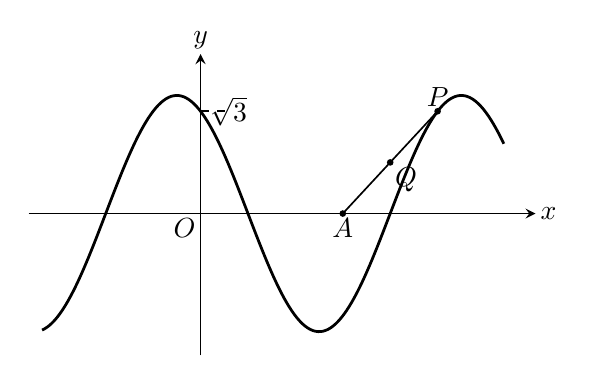
\begin{tikzpicture}[x=1.15cm, y=0.75cm, semithick,
  every node/.style={inner sep=1.5pt}]

  \draw[->,>=stealth] (-1.9,0) -- (3.7,0) node[right] {$x$};
  \draw[->,>=stealth] (0,-2.4) -- (0,2.7) node[above] {$y$};
  \node[below left] at (0,0) {$O$};

  \draw[domain=-1.75:3.35,samples=180,line width=1pt]
    plot (\x,{2*cos(deg(2*\x + pi/6))});

  \coordinate (A) at (1.5708,0);
  \coordinate (Q) at (2.0944,0.8660);
  \coordinate (P) at (2.6180,1.7320);

  \draw (A) -- (P);
  \fill (A) circle (1.2pt);
  \fill (Q) circle (1.2pt);
  \fill (P) circle (1.2pt);
  \node[below] at (A) {$A$};
  \node[below right] at (Q) {$Q$};
  \node[above] at (P) {$P$};

  % y 轴上的 √3 标记
  \draw[dashed] (0,1.732) -- (0.35,1.732);
  \node[right] at (0.05,1.732) {$\sqrt3$};
\end{tikzpicture}
\end{center}
\nopagebreak[4]
\Needspace{4\baselineskip}
\textbf{解析}

\Needspace{5\baselineskip}
（1）$2\cos\theta=\sqrt3$ 且 $0\leqslant\theta\leqslant\dfrac{\pi}{2}$，故 $\theta=\dfrac{\pi}{6}$。又

\nopagebreak[4]
\[y'=-2\omega\sin(\omega x+\theta),\]

\nopagebreak[4]
\[y'(0)=-2\omega\sin\frac{\pi}{6}=-\omega=-2,\]

故 $\omega=2$。

\Needspace{5\baselineskip}
（2）$P(x_P,y_P)$，$Q$ 为 $PA$ 中点：

\nopagebreak[4]
\[x_P=2x_0-\frac{\pi}{2},\qquad y_P=2y_0=\sqrt3.\]

\Needspace{5\baselineskip}
$P$ 在 $y=2\cos\left(2x+\dfrac{\pi}{6}\right)$ 上：

\nopagebreak[4]
\[\cos\left(4x_0-\frac{5\pi}{6}\right)=\frac{\sqrt3}{2}.\]

\Needspace{5\baselineskip}
于是

\nopagebreak[4]
\[4x_0-\frac{5\pi}{6}=\pm\frac{\pi}{6}+2k\pi.\]

取 $+\dfrac{\pi}{6}$ 得 $x_0=\dfrac{\pi}{4}+\dfrac{k\pi}{2}$，在区间内取 $k=1$ 得 $x_0=\dfrac{3\pi}{4}$；

取 $-\dfrac{\pi}{6}$ 得 $x_0=\dfrac{\pi}{6}+\dfrac{k\pi}{2}$，在区间内取 $k=1$ 得 $x_0=\dfrac{2\pi}{3}$。

\gkanswer{答案：（1）$\theta=\dfrac{\pi}{6}$，$\omega=2$；（2）$x_0=\dfrac{2\pi}{3}$ 或 $\dfrac{3\pi}{4}$。}

\end{answer}
\begin{answer}
\gksolhead{19}{}

\textbf{题目}：

某陶瓷厂准备烧制甲、乙、丙三件不同的工艺品，制作过程中必须先后经过两次烧制，当第一次烧制合格后可进入第二次烧制，两次烧制过程相互独立。根据该厂现有的技术水平，经过第一次烧制后，甲、乙、丙三件产品合格的概率依次为 $0.5$，$0.6$，$0.4$。经过第二次烧制后，甲、乙、丙三件产品合格的概率依次为 $0.6$，$0.5$，$0.75$。

（1）求第一次烧制后恰有一件产品合格的概率；

（2）经过前后两次烧制后，合格工艺品的个数为 $\xi$，求随机变量 $\xi$ 的期望。

\Needspace{4\baselineskip}
\textbf{解析}

\Needspace{5\baselineskip}
（1）恰有一件第一次合格：

\nopagebreak[4]
\[0.5\times0.4\times0.6+0.5\times0.6\times0.6+0.5\times0.4\times0.4=0.12+0.18+0.08=0.38.\]

\Needspace{5\baselineskip}
（2）各件两次都合格的概率：

\nopagebreak[4]
\[p_{\text{\text{甲}}}=0.5\times0.6=0.3,\quad p_{\text{\text{乙}}}=0.6\times0.5=0.3,\quad p_{\text{\text{丙}}}=0.4\times0.75=0.3.\]

\Needspace{5\baselineskip}
由期望的线性性，

\nopagebreak[4]
\[E\xi=0.3+0.3+0.3=0.9.\]

\gkanswer{答案：（1）$0.38$；（2）$E\xi=0.9$。}

\end{answer}
\begin{answer}
\gksolhead{20}{}

\textbf{题目}：

如图是一个直三棱柱（以 $A_1B_1C_1$ 为底面）被一平面所截得到的几何体，截面为 $ABC$。已知 $A_1B_1=B_1C_1=1$，$\angle A_1B_1C_1=90^\circ$，$AA_1=4$，$BB_1=2$，$CC_1=3$。

（1）设点 $O$ 是 $AB$ 的中点，证明：$OC\parallel$ 平面 $A_1B_1C_1$；

（2）求二面角 $B-AC-A_1$ 的大小；

（3）求此几何体的体积。
\nopagebreak[4]
\begin{center}% 2007 年江西卷理科第 20 题：直三棱柱被平面 ABC 截得的几何体。
%   底面 A1B1C1 为等腰直角三角形，AA1=4、BB1=2、CC1=3；O 为 AB 中点。
% 来源 PDF：gaokaomath-src/普通高考/2007/2007江西理.pdf
% SHA-256：6602cbc393b02e9940beb0035be6e2a28d88a77e0e7792260dcd4c873b542a82
% 原页：2007江西理.pdf 第 2 页（A3 三栏）第 1 栏，书页码 386。
% 重绘依据：按原页截棱柱的斜投影与 O、C 的位置重绘。
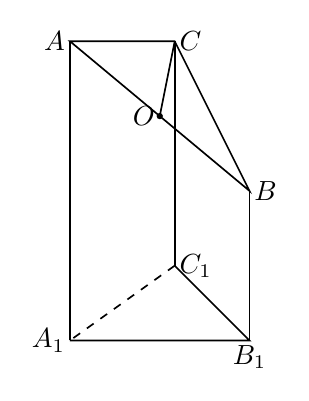
\begin{tikzpicture}[scale=0.95, semithick,
  every node/.style={inner sep=1.5pt}]

  \coordinate (A1) at (0,0);
  \coordinate (B1) at (2.4,0);
  \coordinate (C1) at (1.4,1.0);
  \coordinate (A)  at (0,4.0);
  \coordinate (B)  at (2.4,2.0);
  \coordinate (C)  at (1.4,4.0);
  \coordinate (O)  at (1.2,3.0);

  % 底面
  \draw (A1) -- (B1) -- (C1);
  \draw[dashed] (C1) -- (A1);
  % 侧棱
  \draw (A1) -- (A);
  \draw (B1) -- (B);
  \draw (C1) -- (C);
  % 截面 ABC
  \draw (A) -- (B) -- (C) -- cycle;
  % O 与 OC
  \fill (O) circle (1.2pt);
  \draw (O) -- (C);

  \node[left] at (A) {$A$};
  \node[right] at (B) {$B$};
  \node[right] at (C) {$C$};
  \node[left] at (A1) {$A_1$};
  \node[below] at (B1) {$B_1$};
  \node[right] at (C1) {$C_1$};
  \node[left] at (O) {$O$};
\end{tikzpicture}
\end{center}
\nopagebreak[4]
\Needspace{4\baselineskip}
\textbf{解析}

建系同文科卷，取底面三点 $B_1(0,0,0)$、$A_1(1,0,0)$、$C_1(0,1,0)$。

其余各点为 $A(1,0,4)$、$B(0,0,2)$、$C(0,1,3)$、$O\left(\dfrac12,0,3\right)$。

（1）$\overrightarrow{OC}=\left(-\dfrac12,1,0\right)$，其 $z$ 分量为 $0$，平行于底面 $A_1B_1C_1$；又 $O$ 不在底面内，故 $OC\parallel$ 平面 $A_1B_1C_1$。

\Needspace{5\baselineskip}
（2）平面 $ABC$ 的法向量：$\overrightarrow{AB}=(-1,0,-2)$，$\overrightarrow{AC}=(-1,1,-1)$，

\nopagebreak[4]
\[\boldsymbol n_1=\overrightarrow{AB}\times\overrightarrow{AC}=(2,1,-1).\]

\Needspace{5\baselineskip}
平面 $AA_1C$ 的法向量：$\overrightarrow{AA_1}=(0,0,-4)$，$\overrightarrow{AC}=(-1,1,-1)$，

\nopagebreak[4]
\[\boldsymbol n_2=\overrightarrow{AA_1}\times\overrightarrow{AC}=(4,4,0)\sim(1,1,0).\]

\Needspace{5\baselineskip}
设二面角为 $\theta$，则

\nopagebreak[4]
\[\cos\theta=\frac{|\boldsymbol n_1\cdot\boldsymbol n_2|}{|\boldsymbol n_1||\boldsymbol n_2|}=\frac{3}{\sqrt6\cdot\sqrt2}=\frac{\sqrt3}{2},\]

故 $\theta=30^\circ$。

\Needspace{5\baselineskip}
（3）底面积 $\dfrac12$，截面平面 $z=2x+y+2$ 在底面重心 $\left(\dfrac13,\dfrac13,0\right)$ 处的高为 $3$，故

\nopagebreak[4]
\[V=\frac12\times3=\frac32.\]

\gkanswer{答案：（1）证明见解析；（2）$30^\circ$；（3）$\dfrac32$。}

\end{answer}
\begin{answer}
\gksolhead{21}{}

\textbf{题目}：

设动点 $P$ 到点 $A(-1,0)$ 和 $B(1,0)$ 的距离分别为 $d_1$ 和 $d_2$，$\angle APB=2\theta$，且存在常数 $\lambda$（$0<\lambda<1$），使得 $d_1d_2\sin^2\theta=\lambda$。

（1）证明：动点 $P$ 的轨迹 $C$ 为双曲线，并求出 $C$ 的方程；

（2）过点 $B$ 作直线交双曲线 $C$ 的右支于 $M$，$N$ 两点，试确定 $\lambda$ 的范围，使 $\overrightarrow{OM}\cdot\overrightarrow{ON}=0$，其中点 $O$ 为坐标原点。
\nopagebreak[4]
\begin{center}% 2007 年江西卷理科第 21 题：动点 P 到 A(-1,0)、B(1,0) 的距离 d1、d2，
%   ∠APB=2θ；图中标出 d1、d2 与 2θ。
% 来源 PDF：gaokaomath-src/普通高考/2007/2007江西理.pdf
% SHA-256：7c0b4b6681b5d98c71dcaab52445896ece61e7a8113032234967c415ef3c0ab1
% 原页：2007江西理.pdf 第 2 页（A3 三栏）第 2 栏，书页码 386。
% 重绘依据：按原页 A、O、B、P 与两条距离线、角 2θ 的位置重绘。
\begin{tikzpicture}[scale=1.0, semithick,
  every node/.style={inner sep=1.5pt}]

  \draw[->,>=stealth] (-2.2,0) -- (3.0,0) node[right] {$x$};
  \draw[->,>=stealth] (0,-1.8) -- (0,2.6) node[above] {$y$};
  \node[below left] at (0,0) {$O$};

  \coordinate (A) at (-1,0);
  \coordinate (B) at (1,0);
  \coordinate (P) at (1.8,1.5);

  \draw (P) -- (A);
  \draw (P) -- (B);
  \fill (A) circle (1.2pt);
  \fill (B) circle (1.2pt);
  \fill (P) circle (1.2pt);

  \node[below] at (A) {$A$};
  \node[below] at (B) {$B$};
  \node[above right] at (P) {$P$};
  \node[left] at (0.35,0.85) {$d_1$};
  \node[right] at (1.45,0.8) {$d_2$};
  \node at (1.35,1.15) {$2\theta$};
\end{tikzpicture}
\end{center}
\nopagebreak[4]
\Needspace{4\baselineskip}
\textbf{解析}

\Needspace{5\baselineskip}
（1）在 $\triangle APB$ 中，$AB=2$，由余弦定理：

\nopagebreak[4]
\[4=d_1^2+d_2^2-2d_1d_2\cos2\theta.\]

\Needspace{5\baselineskip}
利用 $\cos2\theta=1-2\sin^2\theta$：

\nopagebreak[4]
\[4=(d_1-d_2)^2+4d_1d_2\sin^2\theta=(d_1-d_2)^2+4\lambda.\]

\Needspace{5\baselineskip}
故

\nopagebreak[4]
\[|d_1-d_2|=2\sqrt{1-\lambda},\]

\Needspace{5\baselineskip}
为小于 $2$ 的常数。由双曲线定义，$P$ 的轨迹是以 $A$，$B$ 为焦点、实半轴 $a=\sqrt{1-\lambda}$ 的双曲线。半焦距 $c=1$，虚半轴

\nopagebreak[4]
\[b^2=c^2-a^2=\lambda,\]

\Needspace{5\baselineskip}
故

\nopagebreak[4]
\[C:\ \frac{x^2}{1-\lambda}-\frac{y^2}{\lambda}=1.\]

\Needspace{5\baselineskip}
（2）设过 $B(1,0)$ 的直线为

\nopagebreak[4]
\[y=k(x-1).\]

\Needspace{5\baselineskip}
代入双曲线方程：

\nopagebreak[4]
\[\frac{x^2}{1-\lambda}-\frac{k^2(x-1)^2}{\lambda}=1.\]

\Needspace{5\baselineskip}
整理得

\nopagebreak[4]
\[[\lambda-k^2(1-\lambda)]x^2+2k^2(1-\lambda)x-k^2(1-\lambda)-\lambda(1-\lambda)=0.\]

\Needspace{5\baselineskip}
设交点为 $M(x_1,y_1)$，$N(x_2,y_2)$。由韦达定理可得 $x_1+x_2$，$x_1x_2$。条件

\nopagebreak[4]
\[\overrightarrow{OM}\cdot\overrightarrow{ON}=0\]

\Needspace{5\baselineskip}
即

\nopagebreak[4]
\[x_1x_2+y_1y_2=0.\]

\Needspace{5\baselineskip}
又 $y_i=k(x_i-1)$，故

\nopagebreak[4]
\[(1+k^2)x_1x_2-k^2(x_1+x_2)+k^2=0.\]

\Needspace{5\baselineskip}
代入韦达定理化简得

\nopagebreak[4]
\[k^2=\frac{\lambda(1-\lambda)}{\lambda^2+\lambda-1}.\]

\Needspace{5\baselineskip}
要求 $k^2>0$，需

\nopagebreak[4]
\[\lambda^2+\lambda-1>0\ \Rightarrow\ \lambda>\frac{\sqrt5-1}{2}.\]

\Needspace{5\baselineskip}
又直线与右支有两个交点，需斜率绝对值大于渐近线斜率 $\dfrac{b}{a}=\sqrt{\dfrac{\lambda}{1-\lambda}}$：

\nopagebreak[4]
\[k^2>\frac{\lambda}{1-\lambda}.\]

\Needspace{5\baselineskip}
代入 $k^2$ 化简易得

\nopagebreak[4]
\[\lambda<\frac23.\]

\Needspace{5\baselineskip}
综上，

\nopagebreak[4]
\[\frac{\sqrt5-1}{2}<\lambda<\frac23.\]

\gkanswer{答案：（1）$\dfrac{x^2}{1-\lambda}-\dfrac{y^2}{\lambda}=1$；（2）$\dfrac{\sqrt5-1}{2}<\lambda<\dfrac23$。}

\end{answer}